\documentclass[11pt,letterpaper]{article}
\usepackage[margin=1in]{geometry}
\usepackage[T1]{fontenc}
\usepackage[utf8]{inputenc}
\usepackage{lmodern}
\usepackage{amsmath,amssymb}
\usepackage{array}
\usepackage{booktabs}
\usepackage{graphicx}
\usepackage{hyperref}
\usepackage{xcolor}

\newcommand{\term}[1]{\textcolor{blue}{#1}}
% State spaces: real (historically realized) vs conceivable (all possible) foods
\newcommand{\RealFoods}{\mathbb{F}_{\mathrm{real}}}
\newcommand{\ConceivableFoods}{\mathbb{F}_{\infty}}

\title{A Tensor-Based Expansion of the Cube Rule for Generative Nutrient Morphology}
\author{Jane Lydia Adams}
\date{\today}

\begin{document}
\pagenumbering{gobble}

\maketitle

\begin{abstract}
We introduce a rigorously parameterized culinary formalism in which edible artifacts are embedded in a third-order nutrient tensor $T \in \{0,1\}^{I \times J \times K}$ spanning cube morphology (index $i$), protein taxonomy ($j$), and starch substrate ($k$).
By recasting food morphology as a coordinate geometry problem over $(i,j,k)$, our framework enables reproducible placement of canonical Cube Rule foods, detection of topological collisions among semantically distinct meals at the same cell, and principled synthesis of plausible-but-previously-unobserved comestible configurations for vacant cells $(i,j,k)$ with $T_{i,j,k}=0$.
To operationalize this framework, we formulate a constrained generative procedure that samples candidate meals for empty cells, enforces axis-consistency invariants on $i$, $j$, $k$ under rejection, and ranks surviving specimens via a composite objective over culinary coherence and novelty.
\end{abstract}

\section{Introduction}

This project studies a formal extension of the Cube Rule of Food, a morphology-based framework originating in Phosphatide's ``Grand Unified Theory of Food Identification''~\cite{phosphatide_gutfi} and later popularized and expanded by André Arko at \url{https://cuberule.com/}~\cite{arko_cube_rule_food}, using a rank-3 tensor $T$ over three categorical axes.
The immediate objective is to define a compact ontology in which each food is assigned a coordinate triple $(i,j,k)$ in the discrete latent space $\{1,\ldots,I\} \times \{1,\ldots,J\} \times \{1,\ldots,K\}$, so that canonical Cube Rule examples are representable and ambiguous cases are explicit.
Our framing treats occupancy, sparsity, and ambiguity as geometric properties of $T$ rather than anecdotal judgments.
Under this formulation, cuisine is represented as a discrete structure over the index space rather than as an informal list of examples.

\subsection{The Cube Rule of Food}

The Cube Rule of Food is a morphology-based classification scheme that assigns a dish according to where structural starch appears on the six faces of an idealized cube. The core idea originates with Phosphatide's ``Grand Unified Theory of Food Identification''~\cite{phosphatide_gutfi}, while the Cube Rule formulation used here follows the later presentation and elaboration by André Arko~\cite{arko_cube_rule_food}.
In the original Rule, these labels are morphology-only categories rather than cuisine names: \emph{salad} has no structural starch faces, \emph{toast} has a bottom starch face, \emph{sandwich} has top and bottom starch faces, \emph{taco} has left, right, and bottom starch faces, \emph{sushi} has top, left, right, and bottom starch faces, \emph{quiche} has side walls and a bottom with an open top, \emph{calzone} is fully enclosed, \emph{cake} consists of stacked starch layers, and \emph{nachos} denotes an outer container plus interior starch pieces.
Some of the Rule's most memorable examples are notably surprising: nigiri counts as \emph{toast}, an Uncrustable counts as \emph{calzone}, and a salad with croutons counts as \emph{nachos}; for the lettuce-crouton boundary case discussed later, see Figure~\ref{fig:horseshoe-salad}.
These nine morphologies define the cube-type axis used throughout this paper and supply the structural vocabulary that the tensor formalism extends with protein and starch-type axes.
Figure~\ref{fig:cube-rule-types} adapts the Cube Rule morphology diagram in schematic form from Arko's presentation~\cite{arko_cube_rule_food}, itself an adaptation and popularization of Phosphatide's original post~\cite{phosphatide_gutfi}.
\begin{figure*}[!tb]
\centering
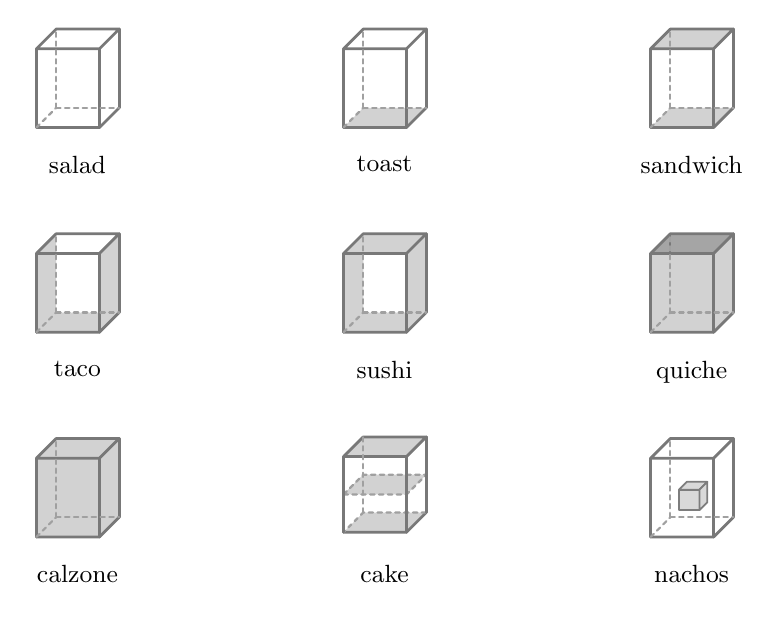
\begin{tikzpicture}[x=1cm,y=1cm,line cap=round,line join=round,font=\small]
\definecolor{starchfill}{RGB}{210,210,210}
\definecolor{starchinner}{RGB}{165,165,165}
\definecolor{starchdark}{RGB}{125,125,125}
\definecolor{wiregray}{RGB}{120,120,120}

\newcommand{\cubehidden}{
  \draw[wiregray!70, dash pattern=on 1.6pt off 1.6pt, line width=0.28mm]
    (0.20,0.00) -- (0.45,0.25);
  \draw[wiregray!70, dash pattern=on 1.6pt off 1.6pt, line width=0.28mm]
    (0.45,0.25) -- (1.25,0.25);
  \draw[wiregray!70, dash pattern=on 1.6pt off 1.6pt, line width=0.28mm]
    (0.45,0.25) -- (0.45,1.25);
}

\newcommand{\cubevisible}{
  \draw[wiregray, line width=0.35mm] (0.20,0.00) -- (1.00,0.00) -- (1.25,0.25);
  \draw[wiregray, line width=0.35mm] (0.20,0.00) -- (0.20,1.00);
  \draw[wiregray, line width=0.35mm] (1.00,0.00) -- (1.00,1.00);
  \draw[wiregray, line width=0.35mm] (1.25,0.25) -- (1.25,1.25);
  \draw[wiregray, line width=0.35mm] (0.20,1.00) -- (1.00,1.00) -- (1.25,1.25) -- (0.45,1.25) -- cycle;
}

\newcommand{\fillbottom}{
  \fill[starchfill]
    (0.20,0.00) -- (1.00,0.00) -- (1.25,0.25) -- (0.45,0.25) -- cycle;
}

\newcommand{\filltop}{
  \fill[starchfill]
    (0.20,1.00) -- (1.00,1.00) -- (1.25,1.25) -- (0.45,1.25) -- cycle;
}

\newcommand{\fillleft}{
  \fill[starchfill]
    (0.20,0.00) -- (0.45,0.25) -- (0.45,1.25) -- (0.20,1.00) -- cycle;
}

\newcommand{\fillright}{
  \fill[starchfill]
    (1.00,0.00) -- (1.25,0.25) -- (1.25,1.25) -- (1.00,1.00) -- cycle;
}

\newcommand{\fillfront}{
  \fill[starchfill]
    (0.20,0.00) -- (1.00,0.00) -- (1.00,1.00) -- (0.20,1.00) -- cycle;
}

\newcommand{\iconlabel}[1]{
  \node[anchor=north,font=\small] at (0.72,-0.24) {#1};
}

\begin{scope}[shift={(0.0,4.3)}]
  \cubevisible
  \cubehidden
  \iconlabel{salad}
\end{scope}

\begin{scope}[shift={(3.9,4.3)}]
  \fillbottom
  \cubevisible
  \cubehidden
  \iconlabel{toast}
\end{scope}

\begin{scope}[shift={(7.8,4.3)}]
  \fillbottom
  \filltop
  \cubevisible
  \cubehidden
  \iconlabel{sandwich}
\end{scope}

\begin{scope}[shift={(0.0,1.7)}]
  \fillbottom
  \fillleft
  \fillright
  \cubevisible
  \cubehidden
  \iconlabel{taco}
\end{scope}

\begin{scope}[shift={(3.9,1.7)}]
  \fillbottom
  \fillleft
  \fillright
  \filltop
  \cubevisible
  \cubehidden
  \iconlabel{sushi}
\end{scope}

\begin{scope}[shift={(7.8,1.7)}]
  \fillbottom
  \fillleft
  \fillright
  \fillfront
  \begin{scope}
    \clip (0.20,1.00) -- (1.00,1.00) -- (1.25,1.25) -- (0.45,1.25) -- cycle;
    \fill[starchinner]
      (0.20,1.00) -- (0.45,1.00) -- (0.45,1.25) -- cycle;
    \fill[starchinner]
      (0.45,1.00) -- (1.00,1.00) -- (1.25,1.25) -- (0.45,1.25) -- cycle;
    \draw[wiregray, line width=0.28mm] (0.45,1.00) -- (0.45,1.25);
  \end{scope}
  \cubevisible
  \cubehidden
  \iconlabel{quiche}
\end{scope}

\begin{scope}[shift={(0.0,-0.9)}]
  \fillbottom
  \fillleft
  \fillright
  \fillfront
  \filltop
  \cubevisible
  \cubehidden
  \iconlabel{calzone}
\end{scope}

\begin{scope}[shift={(3.9,-0.9)}]
  \fill[starchfill]
    (0.20,0.06) -- (1.00,0.06) -- (1.25,0.31) -- (0.45,0.31) -- cycle;
  \fill[starchfill]
    (0.20,0.54) -- (1.00,0.54) -- (1.25,0.79) -- (0.45,0.79) -- cycle;
  \fill[starchfill]
    (0.20,1.02) -- (1.00,1.02) -- (1.25,1.27) -- (0.45,1.27) -- cycle;
  \draw[wiregray, line width=0.35mm] (0.20,0.06) -- (1.00,0.06) -- (1.25,0.31);
  \draw[wiregray!70, dash pattern=on 1.6pt off 1.6pt, line width=0.28mm]
    (1.25,0.31) -- (0.45,0.31) -- (0.20,0.06);
  \draw[wiregray!70, dash pattern=on 1.6pt off 1.6pt, line width=0.28mm]
    (0.20,0.54) -- (1.00,0.54) -- (1.25,0.79) -- (0.45,0.79) -- cycle;
  \draw[wiregray, line width=0.35mm] (0.20,1.02) -- (1.00,1.02) -- (1.25,1.27) -- (0.45,1.27) -- cycle;
  \draw[wiregray, line width=0.35mm] (0.20,0.06) -- (0.20,1.02);
  \draw[wiregray, line width=0.35mm] (1.00,0.06) -- (1.00,1.02);
  \draw[wiregray, line width=0.35mm] (1.25,0.31) -- (1.25,1.27);
  \draw[wiregray!70, dash pattern=on 1.6pt off 1.6pt, line width=0.28mm]
    (0.45,0.31) -- (0.45,1.27);
  \iconlabel{cake}
\end{scope}

\begin{scope}[shift={(7.8,-0.9)}]
  \cubevisible
  \cubehidden
  \filldraw[fill=starchfill!85!white, draw=starchdark, line width=0.22mm]
    (0.56,0.34) -- (0.82,0.34) -- (0.82,0.60) -- (0.56,0.60) -- cycle;
  \filldraw[fill=starchfill!85!white, draw=starchdark, line width=0.22mm]
    (0.56,0.60) -- (0.82,0.60) -- (0.92,0.70) -- (0.66,0.70) -- cycle;
  \filldraw[fill=starchfill!85!white, draw=starchdark, line width=0.22mm]
    (0.82,0.34) -- (0.92,0.44) -- (0.92,0.70) -- (0.82,0.60) -- cycle;
  \iconlabel{nachos}
\end{scope}
\end{tikzpicture}
\caption{Cube-type morphology schematics for the nine categories on axis $i$, adapted from Arko's Cube Rule presentation~\cite{arko_cube_rule_food}, itself adapted from Phosphatide's original ``Grand Unified Theory of Food Identification'' post~\cite{phosphatide_gutfi}. The shaded regions indicate structural starch placement; the drawings are schematic rather than literal geometric reconstructions.}
\label{fig:cube-rule-types}
\end{figure*}


\section{Related Work}

This work builds on the Cube Rule as a prior food-classification framework and introduces two external strands of literature to formalize the proposed tensor-based approach.
The first strand is modern LLM control and prompting: \term{prompt taxonomies}, \term{schema-constrained generation}, \term{grammar-constrained decoding}, \term{guided decoding}, and \term{retrieval-augmented generation} provide language for the prompt design, structured decoding, exemplar use, and post-generation filtering described in the Methods section.
The second strand is tensor and geometry-oriented representation theory: \term{tensor completion}, \term{manifold hypothesis}, \term{simplicial complex} constructions, \term{persistent homology}, and \term{topological data analysis} provide language for discussing empty-cell completion, clustered occupancy structure, and topological features of the support set $\mathcal{S} = \{(i,j,k) : T_{i,j,k}=1\}$ in higher-order categorical space.
Classical combinatorics references are also relevant for occupancy guarantees, including direct pigeonhole-style collision arguments when the number of foods exceeds $|I \times J \times K| = IJK$.
Taken together, these literatures provide the methodological and conceptual vocabulary used to define, populate, and analyze the proposed taxonomy.

\section{Methods}

We define two state spaces in direct analogy to the real numbers $\mathbb{R}$ (the space of all real numbers).
Let $\RealFoods$ denote the \emph{theoretical} set of all \emph{real} foods: those taken to have been cooked and recorded in history (the culinary analogue of ``real'' in $\mathbb{R}$); we approximate this set with our catalog rather than observe it in full.
Let $\ConceivableFoods$ denote the \emph{theoretical} set of all \emph{conceivable} foods, including in principle dishes that have never been prepared---the full state space of possible foods, which we cannot directly verify---with $\RealFoods \subseteq \ConceivableFoods$.
Our tensor formalism maps elements of $\ConceivableFoods$ to coordinates; the catalog we maintain is a finite subset of $\RealFoods$, and we speculate over elements of $\ConceivableFoods \setminus \RealFoods$ for empty cells.

Let $T \in \{0,1\}^{I \times J \times K}$ denote a tensor indexed by cube type (axis $i \in \{1,\ldots,I\}$), protein class (axis $j \in \{1,\ldots,J\}$), and starch type (axis $k \in \{1,\ldots,K\}$).
The starch axis includes a distinguished \texttt{none} value for dishes with no structural starch substrate.
We set $T_{i,j,k}=1$ when at least one food maps to index triple $(i,j,k)$; the \emph{support set} (or, in less restrained prose, the Standard Meal Set) is $\mathcal{S} = \{(i,j,k) : T_{i,j,k}=1\}$ and the set of \emph{empty cells} is $\mathcal{E} = \{(i,j,k) : T_{i,j,k}=0\}$.
In implementation, each occupied cell may contain multiple candidate foods, so the data pipeline stores per-food records and derives occupancy from those records; formally we retain binary $T_{i,j,k}$ while allowing multiple foods per $(i,j,k)$ in the database.
This can be interpreted as a categorical incidence tensor with sparse $|\mathcal{S}| \ll IJK$: for example, cells for nigiri, burritos, ramen, and cheesecake may be occupied while many nearby combinations remain empty.
Operationally, this turns informal culinary intuition into an explicit indexed representation.
\begin{figure}[!tb]
\centering
\tdplotsetmaincoords{68}{118}
\begin{tikzpicture}[tdplot_main_coords, scale=1.1, line cap=round, line join=round, >=Latex]
\definecolor{tensorblue}{RGB}{105,105,105}
\definecolor{tensorfill}{RGB}{210,210,210}
\definecolor{tensorgray}{RGB}{90,90,90}
\tikzset{
  tensorborder/.style={
    draw=tensorgray,
    dash pattern=on 1.6pt off 1.6pt,
    line width=0.32mm
  }
}

\coordinate (O) at (0,0,0);
\coordinate (X) at (4,0,0);
\coordinate (Y) at (0,3.2,0);
\coordinate (Z) at (0,0,3);
\coordinate (XY) at (4,3.2,0);
\coordinate (XZ) at (4,0,3);
\coordinate (YZ) at (0,3.2,3);
\coordinate (XYZ) at (4,3.2,3);

\filldraw[fill=tensorfill, fill opacity=0.22, draw=tensorblue!75]
  (O) -- (X) -- (XY) -- (Y) -- cycle;
\filldraw[fill=tensorfill, fill opacity=0.12, draw=tensorblue!70]
  (O) -- (X) -- (XZ) -- (Z) -- cycle;
\filldraw[fill=tensorfill, fill opacity=0.16, draw=tensorblue!70]
  (X) -- (XY) -- (XYZ) -- (XZ) -- cycle;

\draw[tensorborder] (O) -- (X);
\draw[tensorborder] (X) -- (XY);
\draw[tensorborder] (O) -- (Y);
\draw[tensorborder] (O) -- (Z);
\draw[tensorborder] (Y) -- (YZ);
\draw[tensorborder] (X) -- (XZ);
\draw[tensorborder] (XY) -- (XYZ);
\draw[tensorborder] (Z) -- (XZ) -- (XYZ) -- (YZ) -- cycle;

\draw[->, thick] (O) -- (4.65,0,0) node[anchor=west, xshift=5pt, yshift=-4pt] {$i$ (cube type)};
\draw[->, thick] (O) -- (0,3.75,0) node[anchor=south, xshift=4pt, yshift=4pt] {$j$ (protein)};
\draw[->, thick] (O) -- (0,0,3.55) node[anchor=south] {$k$ (starch)};

\foreach \p in {(0.55,2.25,0.65),(1.35,0.95,2.1),(2.85,2.55,0.55),(3.1,1.15,2.45),(2.15,1.7,1.0)} {
  \fill[tensorgray] \p circle (1.15pt);
}

\coordinate (P) at (2.35,1.65,1.55);
\filldraw[fill=white, draw=black, line width=0.25mm] (P) circle (1.55pt);
\node[anchor=west, xshift=6pt, yshift=-3pt] at (2.68,1.65,1.55) {$T_{i,j,k}$};
\end{tikzpicture}
\caption{Tensor schematic. The cube-type, protein, and starch axes define the index space of $T$; filled markers illustrate occupied cells in $\mathcal{S}$, and the highlighted marker indicates a generic cell $(i,j,k)$.}
\label{fig:tensor-axes}
\end{figure}


Under the Cube Rule, salad morphology means no structural starch faces.
In the tensor, such cases occupy the slice $(i_{\text{salad}}, j, k_{\text{none}})$.
A dish that contains structural starch (e.g., a salad with croutons) is reclassified as nachos (outer container plus inner starch), not salad.
Admissible cells therefore satisfy the compatibility condition
\[
  i = i_{\text{salad}} \iff k = k_{\text{none}}.
\]
In words, a cell has salad morphology if and only if it has \texttt{starch\_type=none}.
Figure~\ref{fig:cube-rule-types} in the Introduction summarizes the nine cube-type morphologies used on axis $i$.

\subsection{The Rice Exception, Mono-Foods, and Dish-Level Classification}

The Cube Rule explicitly declines to rule on one case: ``You are free to interpret the nature of rice however you wish.'' It is the only food for which the Rule gives no cube ruling.
The Rule \emph{does} address rice in context: nigiri is toast, sushi rolls are sushi, ramen is nachos.
The ambiguity is thus not rice-in-dishes but \emph{plain rice by itself}---rice as a starch-based mono-food.
The Rule's nachos examples (couscous, poutine, ramen) are illustrated with other things mixed in (couscous with add-ins, poutine with cheese and gravy); nachos is thus starch \emph{plus} other components, not a bowl of plain starch alone.
We therefore speculate that the exception applies to the nature of \emph{plain rice alone}, and that a similar ambiguity holds for other starch-based mono-foods: a bowl of plain pita chips, a bowl of bread crumbs---single-starch items with no second component.
\begin{definition}[Measure-zero carbs]
A mono-starch food occupies a set of culinary measure zero in the space of toppings, but remains topologically nontrivial.
\end{definition}

If one follows the Rule's existing commitments literally, then plain starches by themselves appear to behave like \emph{salads}: mashed potatoes are classified as salad (with soup treated as wet salad), and a similar logic would make a bowl of croutons salad as well. This yields a gradient from salad to nachos with the addition of more things: lettuce with no croutons is salad; lettuce with croutons is nachos; but a bowl of croutons alone reverts to salad because it is again a single food.
Here and throughout, when we discuss mono-food ambiguity we mean starch-based mono-foods such as plain rice or a bowl of croutons; starchless mono-foods are already salad under the ontology (with soup treated as wet salad).
In analogy to the horseshoe theory of political economy---where the far left and far right are argued to resemble each other more than either resembles the center~\cite{horseshoe}---we suggest this be considered the horseshoe theory of salad: the extremes (all lettuce or all croutons) are both salad, while the middle (lettuce and croutons together) is nachos (Figures~\ref{fig:horseshoe-salad} and \ref{fig:horseshoe-salad-ternary}); in the standard lettuce-centered telling, this is simply the Horseshoe Theory of Lettuce.
\begin{figure}[!tb]
\centering
\includegraphics[width=\linewidth]{../results/figures/lettuce_croutons_gradient.png}
\caption{Horseshoe theory of salad: percent lettuce vs.\ percent croutons. The extremes $(0,100)$ and $(100,0)$ are salad (single component); the middle $(50,50)$ is nachos. Dotted line: lettuce-crouton proportion gradient.}
\label{fig:horseshoe-salad}
\end{figure}
\begin{figure}[!tb]
\centering
\begin{tikzpicture}
\begin{ternaryaxis}[
  width=0.92\linewidth,
  height=0.80\linewidth,
  clip=false,
  grid=major,
  major grid style={draw=black!25},
  axis line style={draw=black, line width=0.35mm},
  tick style={draw=black},
  tick label style={font=\small, text=black},
  xlabel={\% lettuce},
  ylabel={\% croutons},
  zlabel={\% cheese},
  label style={sloped, font=\normalsize, text=black},
  xmin=0, xmax=1,
  ymin=0, ymax=1,
  zmin=0, zmax=1,
  ternary limits relative=true,
  xtick={0,0.2,0.4,0.6,0.8,1.0},
  ytick={0,0.2,0.4,0.6,0.8,1.0},
  ztick={0,0.2,0.4,0.6,0.8,1.0},
]
\addplot3[
  only marks,
  mark=*,
  mark size=2.7pt,
  color=black,
] coordinates {
  (0,1,0)
};
\addplot3[
  no markers,
  color=black,
  line width=1.0mm,
] coordinates {
  (1,0,0)
  (0,0,1)
};
\node[font=\bfseries\large, fill=white, inner sep=1pt] at (axis cs:0.34,0.33,0.33) {nachos};
\node[font=\normalsize, fill=white, inner sep=1pt] at (axis cs:0.06,0.90,0.04) {salad};
\node[font=\normalsize, fill=white, inner sep=1pt, rotate=-60] at (axis cs:0.52,0.02,0.46) {salad};
\end{ternaryaxis}
\end{tikzpicture}
\caption{Ternary extension of the horseshoe theory of salad over lettuce, croutons, and cheese. The highlighted crouton-free, lettuce-cheese edge is the ternary trace of the keto plane: any combination of lettuce and cheese with croutons fixed at zero remains salad rather than nachos (assuming no new starch is added, such as quinoa). Note that the whole interior region is considered nachos, because any amount of croutons morphologically introduces a small amount of starch enclosed by the outer container. However, in keeping with the logic that mashed potatoes are salad, we consider a dish that is 100\% comprised of croutons to also be salad.}
\label{fig:horseshoe-salad-ternary}
\end{figure}

For the purposes of this paper, we retain the Rule's current dish-level categories and use the horseshoe construction only to describe how mono-starch edge cases behave under the existing ontology. We therefore leave that repair on the back burner and return in the Discussion to whether these cases motivate a new category beyond the present nine.

\subsection{Constrained LLM Candidate Generation}

Cells $(i,j,k) \in \mathcal{E}$ (candidates in $\ConceivableFoods \setminus \RealFoods$) are queried with a morphology-first prompt that includes a compact Cube Rule crash course, type-specific definitions, and canonical Cube Rule examples.
This prompt can be viewed as a small prompt taxonomy: it separates structural morphology instructions, axis-definition instructions, and admissibility constraints so that each part of the classification problem is stated explicitly.
The prompt enforces exact axis matching for cube morphology, protein class, and starch class rather than semantic similarity.
For example, bottom-face-only starch placements are treated as toast morphology even when the dish name is not colloquially ``toast''.
The API call uses schema-constrained generation rather than free-form text parsing: candidates are returned through a tool payload with typed fields (\texttt{shortname}, \texttt{description}, \texttt{is\_real}, \texttt{confidence}, and \texttt{rationale\_brief}).
Operationally, this is also a practical form of grammar-constrained decoding, since only outputs that satisfy the required field structure can be returned; a candidate such as ``cheesecake'' must arrive as a typed row for a specific cell rather than as an essay about dessert.
Prompt instructions also prioritize commonly recognized dish names over compositional labels; when only weak descriptive names are available, the model is instructed to return no candidate.
The inclusion of canonical Cube Rule examples functions as lightweight retrieval-augmented generation: the model is not asked to classify from an unconstrained prior, but from an in-prompt bank of morphology-defining exemplars such as pizza slice, nigiri sushi, burrito, and lasagna.
Prompt scaffolding also states that cube-type labels are morphology-only tags: for example, ``salad'' does not imply a cold dish, and ``taco'' does not imply spice or cuisine identity.
Protein semantics are also made explicit in prompting and filtering: \texttt{none} is reserved for cases without meaningful protein contribution, while dairy ingredients (for example milk, cream, yogurt, and cheese) are treated as dairy-protein signals rather than \texttt{none}.
Accordingly, the canonical Cube Rule flapjacks example is placed at $(i,j,k) = (\texttt{cake}, \texttt{dairy}, \texttt{wheat})$ rather than $(\texttt{toast}, \texttt{none}, \texttt{wheat})$, because the butter sandwiched between layers contributes a meaningful dairy signal; by contrast, a toast sandwich is still a canonical \emph{sandwich} example under the Rule rather than \emph{cake}, since its structure has top and bottom starch faces instead of stacked starch layers with other materials in between~\cite{toast_sandwich}.

\subsection{Model and Cost Disclosure}

All LLM-assisted generation runs used Anthropic Claude (model: \texttt{claude-opus-4-6}).
The total API cost for the full set of reported experiments was \$5.77, generously supported by a grant from the author.

\subsection{Hard Validity Constraints}

The generation prompt includes hard constraints for strict matching:
\begin{itemize}
    \item hard axis-locking on starch type: no starch substitution across classes, so a \texttt{pastry\_dough} cell may admit key lime pie or a Pop-Tart but not falafel pita, quesadilla, or other wheat/corn near-misses;
    \item hard axis-locking on protein type: no protein substitution across classes, so a \texttt{red\_meat} cell may admit spaghetti with meatballs or a burrito but not a falafel wrap, cheesecake, or egg custard tart;
    \item single-entity decoding constraint: no composed ``plate'' outputs that combine separate foods (for example, ``steak with mashed potatoes'' or ``soup served with bread''); the candidate must be one integrated dish rather than a menu pairing;
    \item conservative abstention behavior: if no obvious match exists, the model should return an empty candidate list rather than rationalize a weak fit or invent a strained dish name for the sake of filling the cell.
\end{itemize}
Additionally, cube/starch pairings that violate the structural ontology are prohibited: salad is generated only in the \texttt{starch\_type=none} slice, and non-salad morphologies are generated only with non-\texttt{none} starch types.

These same constraints are enforced after generation using deterministic lexical guardrails, yielding a lightweight constraint-satisfaction layer over candidate rows.
In that sense, the pipeline combines stochastic proposal with guided decoding: the model is steered both at generation time and at acceptance time toward outputs that satisfy the ontology, so structurally invalid salad+starch proposals and plate-style outputs are vetoed before review.
Candidates failing these checks are rejected before they enter the LLM candidate table for downstream review.
Additionally, candidates below a configured confidence threshold are dropped so uncertain guesses do not set $T_{i,j,k} \leftarrow 1$ for speculative $(i,j,k)$.
In brief, candidate proposal is stochastic, but acceptance is governed by deterministic constraints and review.

\subsection{Ground-Truth Calibration}

We validate the filtering pipeline against a ground-truth set derived from canonical Cube Rule examples.
The validation script checks axis mapping consistency and verifies that canonical Cube Rule examples pass the same lexical and protein/starch guardrails used for LLM-generated rows.
During calibration, several false negatives were identified and corrected by refining token matching and conflict rules (for example, avoiding substring-only matches and reducing over-restrictive composition heuristics).
After these adjustments, all canonical Cube Rule examples pass validation under the active guardrail configuration.

\subsection{Visualization Axis Ordering}

For occupancy visualizations, the order of indices on each axis (e.g., which $i$ appears left-to-right) is computed with hierarchical clustering rather than fixed ontology order.
Each index is represented by its binary occupancy profile (e.g., for fixed $i$, the vector $(T_{i,1,1}, \ldots, T_{i,J,K})$ flattened); pairwise dissimilarity is computed with Jaccard distance, and leaves are ordered by average-linkage dendrogram seriation.
This ordering groups indices with similar occupancy structure and is used consistently in both pairwise projections (e.g., $T_{i,j,\cdot}$ over $i,j$) and 3D categorical axes, producing an interpretable occupancy-manifold view of the tensor slices.
At a descriptive level, this reflects a weak manifold hypothesis: foods that are nearby in ontology space, such as nigiri and sushi rolls or salad and nachos edge cases involving croutons, tend to exhibit related occupancy patterns rather than arbitrary dispersion across the tensor.

\section{Experiments}

The experiment workflow has three steps: map observed foods to coordinates $(i,j,k)$ and set $T_{i,j,k}=1$ accordingly; measure occupancy $|\mathcal{S}|$ and collisions (multiple foods at the same $(i,j,k)$); and generate candidate foods for cells in $\mathcal{E}$.
Initial analysis reports which regions of the index set $\{1,\ldots,I\} \times \{1,\ldots,J\} \times \{1,\ldots,K\}$ are dense ($T_{i,j,k}=1$ for many $(i,j,k)$ in a neighborhood), sparse, or structurally inconsistent under the chosen ontology.
From a representation-learning perspective, this is a small-scale study of \term{combinatorial generalization} under hard axis constraints on $i$, $j$, and $k$.
Empirically, the workflow behaves like a controlled stress test of whether culinary naming conventions can survive contact with coordinate geometry.
Axis categories in Figure~\ref{fig:tensor-projections-speculated} and Figure~\ref{fig:tensor-3d-speculated} are ordered by occupancy-profile hierarchical clustering as described in the Methods section (applied to the indices $i$, $j$, $k$ along each axis).
\input{sections/generated/figure_omissions}

\paragraph{Review outcomes.}
All LLM-generated candidates exported for review were accepted and included in the real-only tensor views; the distribution of model confidence for those accepted candidates is shown in Figure~\ref{fig:confidence-histogram}.

We also run a targeted mini-experiment on foods whose names explicitly contain ``salad'' (for example, chicken salad, egg salad, and Snickers salad\footnote{Snickers salad is a dessert-style potluck dish, commonly made with chopped Snickers bars, tart apples, and whipped topping (often with pudding), and is widely associated with Upper Midwest potluck and church-supper traditions (especially Minnesota and Iowa), though no single point of origin is well documented.}), asking the model to classify each item by structural starch placement and thus to assign a cube index $i$ (and implicitly $j$, $k$).
Table~\ref{tab:salad-cube-rule} reports only the subset that violates the Cube Rule salad definition (no structural starch faces; i.e., the assigned $i$ does not match the ``salad'' morphology index).
As a secondary aside experiment, we test the hypothesis that most violations arise from discrete starch inclusions (for example, croutons, pasta pieces, or candy chunks), which shift morphology from the salad index $i_{\text{salad}}$ toward the Cube Rule ``nachos'' index $i_{\text{nachos}}$ (outer dish plus inner starch).
\IfFileExists{sections/generated/salad_cube_rule_table.tex}{%
  \input{sections/generated/salad_cube_rule_table}%
}{%
  \paragraph{Mini-experiment data pending.}
  Run \texttt{uv run python scripts/salad\_cube\_rule\_experiment.py} to generate \texttt{paper/sections/generated/salad\_cube\_rule\_table.tex}.
}

\begin{figure}[t]
\centering
\includegraphics[width=0.49\textwidth]{../results/figures/canonical_plus_llm_identified_plus_llm_speculated/tensor_cube_vs_protein.png}\hfill
\includegraphics[width=0.49\textwidth]{../results/figures/canonical_plus_llm_identified_plus_llm_speculated/tensor_cube_vs_starch.png}
\vspace{0.5em}
\includegraphics[width=0.49\textwidth]{../results/figures/canonical_plus_llm_identified_plus_llm_speculated/tensor_protein_vs_starch.png}
\caption{Pairwise projections of $T$: slices over $(i,j)$, $(i,k)$, and $(j,k)$. Black squares mark canonical $(i,j,k)$ with $T_{i,j,k}=1$, gray squares mark accepted real LLM-identified cells, and white squares with black outlines mark LLM speculative cells; cells in $\mathcal{E}$ are shown without glyphs.\omitSpeculatedSummary}
\label{fig:tensor-projections-speculated}
\end{figure}

\begin{figure}[t]
\centering
\includegraphics[width=0.76\textwidth]{../results/figures/canonical_plus_llm_identified_plus_llm_speculated/tensor_3d.png}
\caption{Static 2D rendering of the 3D occupancy tensor $T$. Black markers indicate canonical $(i,j,k) \in \mathcal{S}$, gray markers indicate accepted real LLM-identified cells, and white markers with black outlines indicate LLM speculative cells; $(i,j,k) \in \mathcal{E}$ are shown without glyphs.}
\label{fig:tensor-3d-speculated}
\end{figure}

\begin{figure}[t]
\centering
\includegraphics[width=0.35\textwidth]{../results/figures/confidence_histogram.png}
\input{sections/generated/confidence_histogram_caption}
\end{figure}

\section{Discussion}

\begin{center}
\fbox{%
\begin{minipage}{0.94\linewidth}
\begin{theorem}[Theorem 1 (No Free Lunch Special).]
If the number of distinct foods assigned to tensor cells exceeds $IJK$, then at least one coordinate $(i,j,k)$ must contain more than one food.
Equivalently, if $|\RealFoods| > IJK$ (or if any subset of $\ConceivableFoods$ of size $> IJK$ is mapped into the index space), then collisions are unavoidable.
\end{theorem}
\begin{proof}[Proof (sketch)]
There are exactly $IJK$ available cells in the tensor.
Assigning more than $IJK$ distinct foods to those cells forces at least one cell to receive two or more foods by the pigeonhole principle~\cite{pigeonhole}.
\end{proof}
\textit{Example.} A concrete collision can occur at $(i,j,k) = (\text{nachos}, \text{red\_meat}, \text{pasta\_noodle})$, where both pasta salad with ground beef and spaghetti with meatballs plausibly occupy the same tensor cell despite differing in serving convention and internal structure.
Such a case suggests that one might introduce a fourth dimension $\ell$ for temperature or a fifth dimension $m$ for protein morphology if finer distinctions are desired.
\end{minipage}%
}
\end{center}

This is mathematically trivial but operationally useful: once the catalog grows past the available cell count, collisions cease to be a modeling accident and become a structural consequence of the ontology.
This motivates optional extensions with additional axes (e.g., a fourth index $\ell$), which can be interpreted as moving from $T \in \{0,1\}^{I \times J \times K}$ toward a higher-order multiway representation.
For example, future work could introduce additional dimensions such as vegetable type (categorical) or spice level (ordinal or quantitative, depending on how pungency is formalized), but doing so would require explicit decisions about data type and measurement scale before such axes could be used to disambiguate colliding items.
One practical tension is model granularity: under-specified ontologies (small $I$, $J$, $K$) collapse semantically distinct foods into the same $(i,j,k)$, while over-specified ontologies create extreme sparsity ($|\mathcal{S}|/IJK$ very small) and weak empirical support per coordinate.
Future extensions should resolve boundary cases where sugar-dominant processed inclusions (for example nougat/candy in Snickers salad) may trigger non-salad intuitions without mapping cleanly to the current starch index $k$.
This paper restricts attention to edible foods, even though the original Cube Rule also discusses non-food cases and famously proposes, for example, that humans are ravioli (that is, calzones under the Rule's morphology).
An expanded ontology with additional starch and protein categories might therefore reveal interesting findings outside ordinary cuisine as well: a leatherbound book, for instance, could be modeled as an inverse taco in which a protein-like exterior surrounds a filling of starch.
We also restrict the morphological axis to ordinary three-dimensional food geometry and do not attempt higher-dimensional morphology.
Future work could ask whether tesseract-like foods or other higher-order culinary solids require an additional extension of the cube axis itself, effectively promoting morphology to a richer higher-dimensional index.
The Cube Rule's rice exception (plain rice as a starch-based mono-food) and the proposed gradient from salad to nachos (single starch $\to$ salad; starch plus other things $\to$ nachos) suggest a possible extension: a dedicated category for \emph{single-starch} foods, distinct from salad and nachos, which would resolve the ``interpret as you wish'' for plain rice, plain croutons, and similar starch-based mono-foods without collapsing them into salad.
Our current dish-level classification leaves that boundary to the Rule's open interpretation.
Relatedly, jello-style dishes suggest that gelatin may warrant a separate protein index $j$ beyond the current formalism, likely yielding a very sparse but interesting subset of $\mathcal{S}$ in the morphological state space (with soup dumplings as one motivating example, since they classify as calzone under Cube Rule morphology and include gelatinized broth).
Topological language is useful here: regions where $T_{i,j,k}=1$ is dense in index space behave like low-curvature neighborhoods, while isolated $(i,j,k) \in \mathcal{S}$ resemble high-curvature outliers in a discrete morphological state space; for example, several bread-based categories may cluster while a more unusual dish such as jello salad sits farther from those neighborhoods.
If local adjacency relations are imposed on occupied cells, $\mathcal{S}$ can also be viewed as inducing a sparse simplicial complex over the index lattice, with missing bridges and cavities corresponding to structurally absent combinations.
Under that view, persistent homology and broader topological data analysis provide language for discussing connected components, holes, and other mesoscale features of the food-occupancy pattern as the ontology grows, such as whether sushi-like foods form one connected region while dessert salads occupy scattered outlier cells.
Operationally, the ontology should avoid both excessive coarseness and excessive fragmentation: $I$, $J$, and $K$ should be large enough to separate distinct dishes, but restrained enough to keep $|\mathcal{S}|$ empirically supportable.

\section{Conclusion}

We have shown that the Cube Rule of Food can be expressed as a geometric classification problem: dishes map to coordinates $(i,j,k)$ in a third-order tensor $T$, with cube morphology $i$, protein taxonomy $j$, and starch substrate $k$ as the axes of a discrete culinary state space.
Canonical Cube Rule examples occupy well-defined cells; empty cells correspond to conceivable-but-unobserved dishes; and collisions---multiple foods at the same $(i,j,k)$---become topological facts rather than matters of taste.
By constraining an LLM to propose candidates under strict axis matching, lexical guardrails, and a review gate, we have extended the support set $\mathcal{S}$ beyond the canonical seed while keeping the tensor falsifiable and the Rule's edge cases explicit: salad occupies the \texttt{starch\_type=none} slice; the rice exception applies to plain rice as a mono-food; and the \term{horseshoe theory of salad} captures the gradient from single-component salad (all lettuce or all croutons) to nachos (lettuce and croutons together).
Methodologically, this combines \term{prompt taxonomies}, lightweight \term{retrieval-augmented generation}, \term{guided decoding}, and constrained \term{tensor completion} within a single food-classification pipeline.

This formalism can also be extended in principled ways.
The index sets $I$, $J$, and $K$ need not remain fixed.
The cube axis $i$ may gain a dedicated \emph{single-starch} category, resolving the Rule's ``interpret as you wish'' for plain rice and bowls of croutons without collapsing them into salad.
The protein axis $j$ may admit gelatin (and thus jello, soup dumplings, and other aspic-bound dishes) as a distinct type, yielding a sparse but coherent region of $\mathcal{S}$.
The starch axis $k$ may be extended to include sugar-dominant substrates---candy, nougat, Snickers bars---so that Snickers salad and its ilk cease to be boundary cases and take their place at a named coordinate.
Such an ontological change, however, should be made with care and with attention to cultural naming practices: doing so would create tension between the Midwestern term ``Snickers salad'' and the strict starch-morphology Cube Rule definition of ``salad,'' potentially opening taxonomic rifts between competing ontologies.
Each such expansion refines the representation of conceivable foods within the same indexing framework.

More broadly, this framework treats morphology, protein, and starch as formal indices rather than informal descriptors.
Future work can therefore extend the same tensor formalism while keeping the convention that salad occupies the \texttt{starch\_type=none} slice, the rice exception, and mono-food boundary cases explicit.


\section*{Acknowledgements}
This work would of course not have been possible without the framework provided by the Cube Rule of Food by André Arko. The author thanks Connor Wilson for inspiring this idea, Michael Davinroy for introducing the concepts of snickers salad and jello salad, and Andrew McNutt for first sharing SIGBOVIK.

\bibliographystyle{plain}
\bibliography{references}

\end{document}
